\documentclass[12pt,a4paper,titlepage,twoside,openright]{article}
\usepackage[english]{babel}
\usepackage{ucs} 
\usepackage[utf8x]{inputenc}
\usepackage[usenames,dvipsnames]{xcolor}
\usepackage{tikz,pgfplots}
\usepackage{tkz-tab}
\usepackage{caption}
\usepackage{latexsym}
\usepackage{amssymb}
\usepackage{amsmath}
\usepackage{subcaption} 

\begin{document}

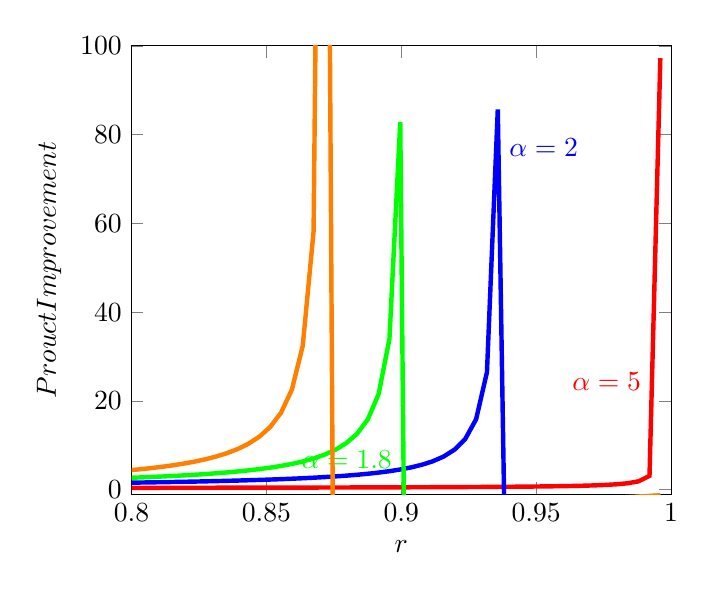
\begin{tikzpicture}
\begin{axis}[ 
xlabel=$r$,
ylabel={$Prouct Improvement$}, xmin=0.8,xmax=1,ymin=-1,ymax=100]

\addplot[domain=0:1,samples=250, ultra thick, red ]{(x+(5-1)*sqrt(1-x))/(4*(5-1)*sqrt(1-x)-1)} node [pos=0.3, below left]{$\alpha = 5$};
\addplot[domain=0:1,samples=250, ultra thick, blue ]{(x+(2-1)*sqrt(1-x))/(4*(2-1)*sqrt(1-x)-1)} node [pos=0.3, below right]{$\alpha = 2$};
\addplot[domain=0:1,samples=250, ultra thick, green ]{(x+(1.8-1)*sqrt(1-x))/(4*(1.8-1)*sqrt(1-x)-1)} node [pos=0.3, below left]{$\alpha = 1.8$};
\addplot[domain=0:1,samples=250, ultra thick, orange ]{(x+(1.7-1)*sqrt(1-x))/(4*(1.7-1)*sqrt(1-x)-1)} node [pos=0.3, below left]{$\alpha = 1.7$};
\end{axis}
\end{tikzpicture}

\end{document}